\documentclass[11pt,a4paper,landscape]{article}
\usepackage[margin=1in]{geometry}
\usepackage{tikz}
\usetikzlibrary{shapes.geometric, arrows.meta, positioning, calc}
\pagestyle{empty}

\begin{document}
\begin{center}
    \textbf{\Large 0-Level DFD: System Context Boundary}\\[10pt]
\end{center}

\begin{center}
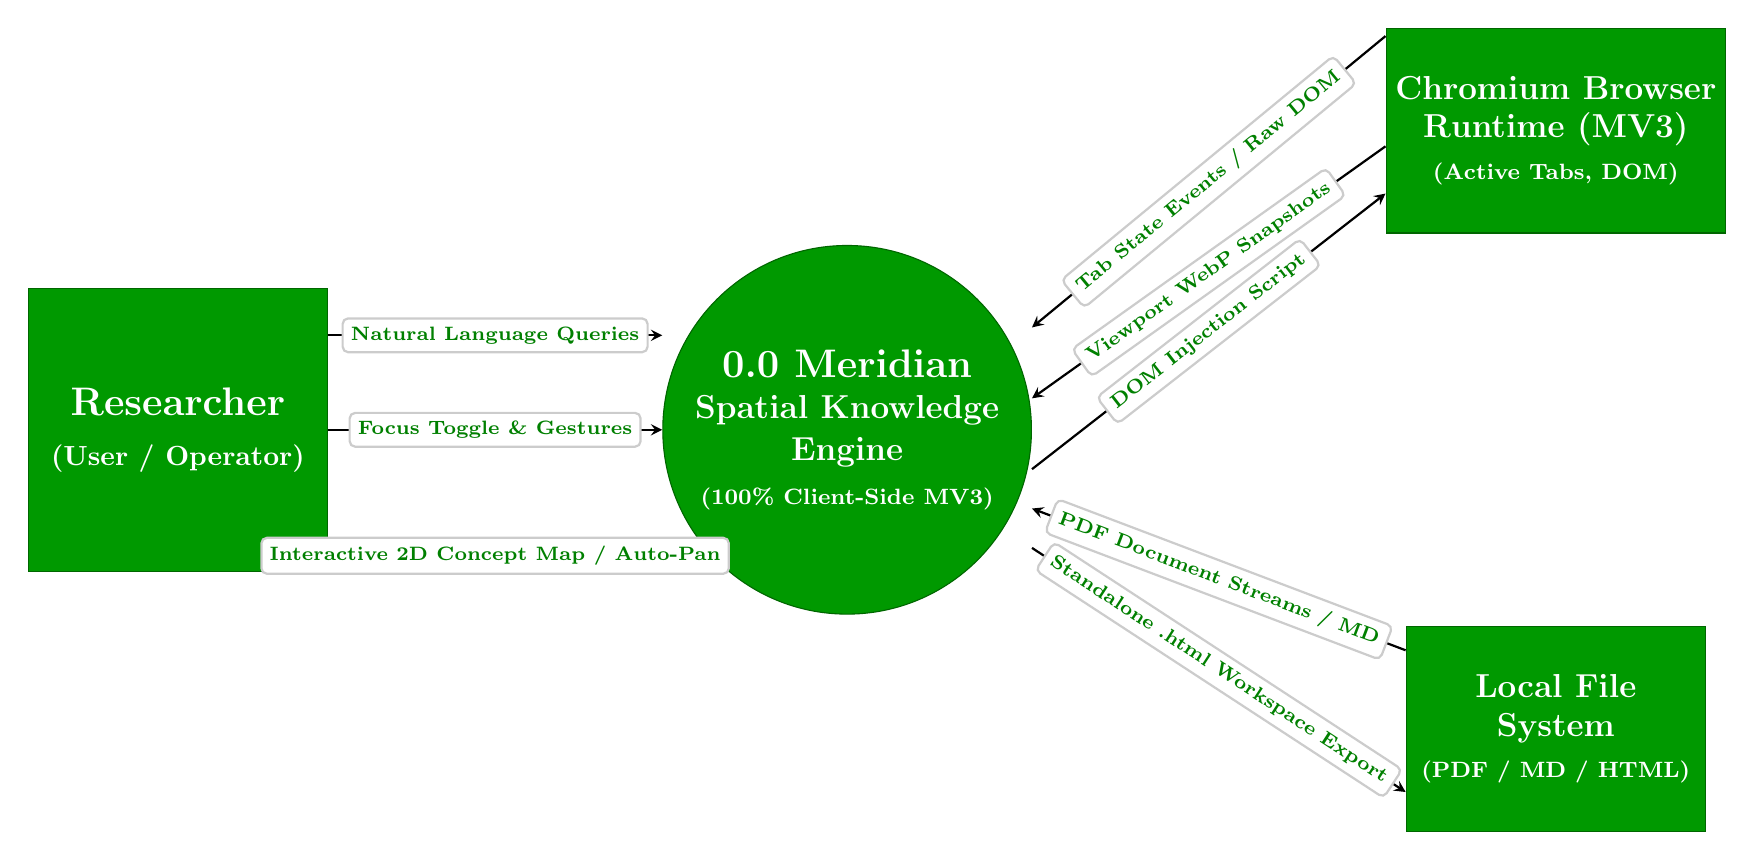
\begin{tikzpicture}[
    font=\sffamily,
    >=stealth,
    % Central Process (0.0 System Circle)
    process0/.style={
        circle, draw=green!40!black, fill=green!60!black, text=white,
        minimum size=4.0cm, align=center, font=\bfseries
    },
    % External Entity Style
    entity/.style={
        rectangle, draw=green!40!black, fill=green!60!black, text=white,
        minimum width=3.8cm, minimum height=2.6cm, align=center, font=\bfseries
    },
    % Flow Annotation Pill Style
    flowlabel/.style={
        fill=white, draw=gray!40, rounded corners=2pt,
        font=\scriptsize\bfseries, text=green!50!black, inner sep=3pt
    }
]

    % =========================================================================
    % Central 0.0 Process
    % =========================================================================
    \node[process0] (p0) at (0,0) {%
        \Large 0.0 Meridian\\[3pt]
        \large Spatial Knowledge\\[3pt]
        \large Engine\\[4pt]
        \footnotesize (100\% Client-Side MV3)
    };

    % =========================================================================
    % External Entities
    % =========================================================================
    % Left Entity: User
    \node[entity, minimum height=3.6cm] (user) at (-8.5, 0) {%
        \Large Researcher\\[6pt]
        \normalsize (User / Operator)
    };

    % Right Top Entity: Browser Runtime
    \node[entity] (browser) at (9.0, 3.8) {%
        \large Chromium Browser\\[2pt]
        \large Runtime (MV3)\\[3pt]
        \footnotesize (Active Tabs, DOM)
    };

    % Right Bottom Entity: Local File System
    \node[entity] (fs) at (9.0, -3.8) {%
        \large Local File\\[2pt]
        \large System\\[3pt]
        \footnotesize (PDF / MD / HTML)
    };

    % =========================================================================
    % Data Flows: User <-> Process 0.0 (Left)
    % =========================================================================
    \draw[->, >=stealth, thick] ([yshift=1.2cm]user.east) -- ([yshift=1.2cm]p0.west) 
        node[midway, flowlabel] {Natural Language Queries};

    \draw[->, >=stealth, thick] ([yshift=0.0cm]user.east) -- ([yshift=0.0cm]p0.west) 
        node[midway, flowlabel] {Focus Toggle \& Gestures};

    \draw[<-, >=stealth, thick] ([yshift=-1.6cm]user.east) -- ([yshift=-1.6cm]p0.west) 
        node[midway, flowlabel] {Interactive 2D Concept Map / Auto-Pan};

    % =========================================================================
    % Data Flows: Process 0.0 <-> Browser Runtime (Top Right)
    % =========================================================================
    \draw[<-, >=stealth, thick] ([yshift=1.3cm]p0.east) -- ([yshift=1.2cm]browser.west) 
        node[midway, flowlabel, sloped] {Tab State Events / Raw DOM};

    \draw[<-, >=stealth, thick] ([yshift=0.4cm]p0.east) -- ([yshift=-0.2cm]browser.west) 
        node[midway, flowlabel, sloped] {Viewport WebP Snapshots};

    \draw[->, >=stealth, thick] ([yshift=-0.5cm]p0.east) -- ([yshift=-0.8cm]browser.west) 
        node[midway, flowlabel, sloped] {DOM Injection Script};

    % =========================================================================
    % Data Flows: Process 0.0 <-> Local File System (Bottom Right)
    % =========================================================================
    \draw[<-, >=stealth, thick] ([yshift=-1.0cm]p0.east) -- ([yshift=1.0cm]fs.west) 
        node[midway, flowlabel, sloped] {PDF Document Streams / MD};

    \draw[->, >=stealth, thick] ([yshift=-1.5cm]p0.east) -- ([yshift=-0.8cm]fs.west) 
        node[midway, flowlabel, sloped] {Standalone .html Workspace Export};

\end{tikzpicture}
\end{center}
\end{document}
